\begin{frame}
    \frametitle{Componentes de segurança em microsserviços}
    \begin{itemize}
        \item \textit{Hardware}  
        \item Virtualização
        \item \textit{Cloud}
        \item Comunicação
        \item \textit{Deployment}
    \end{itemize}    
\end{frame}    

\begin{frame}
    \frametitle{Definição e redefinição do perímetro de segurança}
    \begin{figure}
        \begin{minipage}[c]{0.4\textwidth}
            \centering
            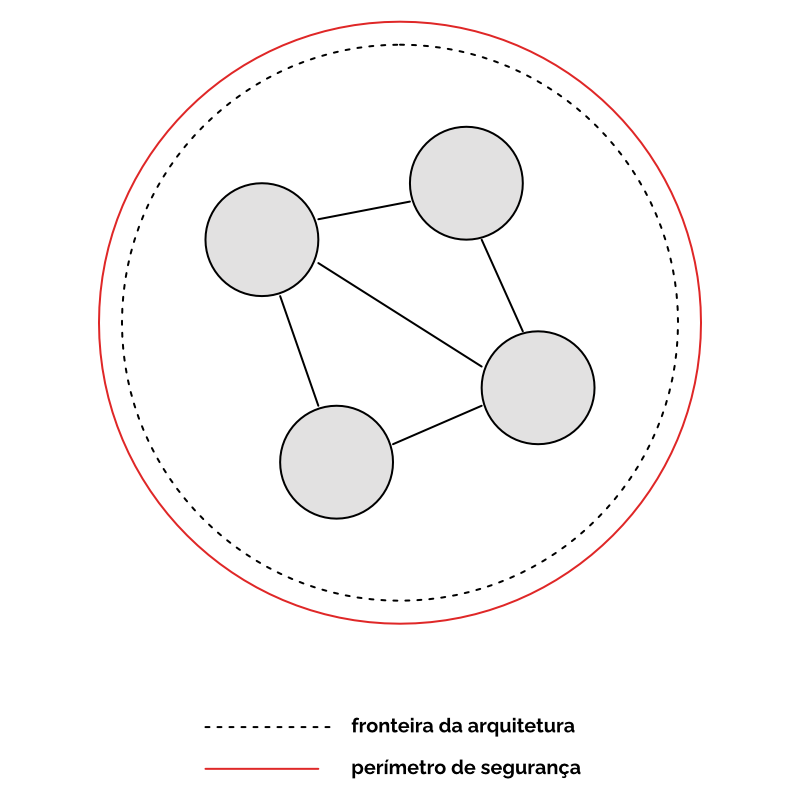
\includegraphics[width=1.2\textwidth]{./assets/seguranca/perimeter_defense.png}
            \caption{\textit{Perimeter defense}} 
        \end{minipage}\hfill
        \begin{minipage}[c]{0.4\textwidth}
            \centering
            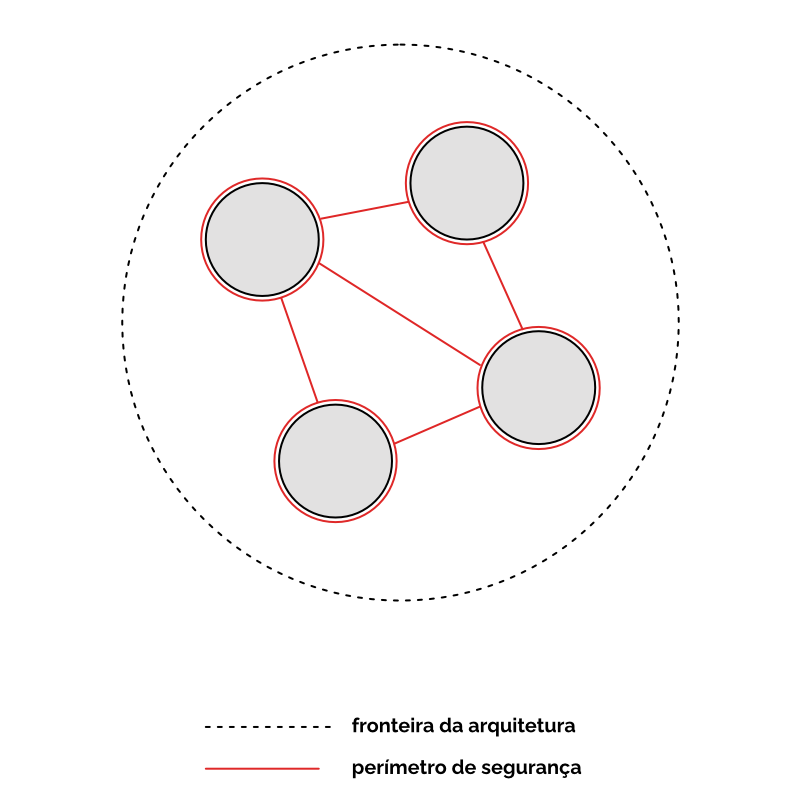
\includegraphics[width=1.2\textwidth]{./assets/seguranca/defense_in_depth.png}
            \caption{\textit{Defense in depth}} 
        \end{minipage}
    \end{figure}
\end{frame}    

\begin{frame}
    \frametitle{Arquitetura com as aprendizagens}
    \begin{figure}
        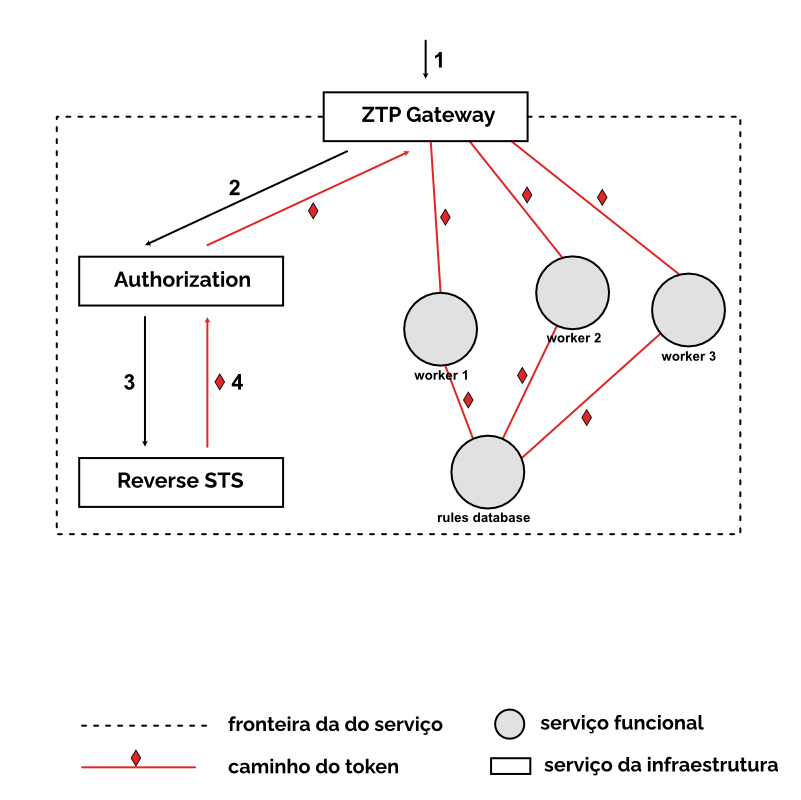
\includegraphics[width=0.7\textwidth]{./assets/seguranca/security_ztp.png}
    \end{figure}
\end{frame}    
